\chapter{Data Analysis}

For the gene expression data set, measured using the \textit{Illumina Human
Ref-8 BeadChips} platform, we applied the TMLE-based biomarker evaluation
procedure to obtain independent estimates of the association of each of the
$\sim 22,000$ biomarkers with benzene exposure, while controlling for potential
confounding based on age, sex, and smoking status. The values obtained from
applying this procedure on a biomarker-by-biomarker basis correspond to the
contributions of each potential biomarker to changes in the ATE, based on the
influence curve decomposition of the ATE parameter. While having a direct
interpretation in relation to the ATE, such transformed expression values hold
little bearing on statistical inference.

Using the ATE, the moderated t-statistic for the test performed is as follows:

$$\tilde{t}_b=\frac{\sqrt[]{n}
(\hat{\Psi}_{b,n}^{A = max(A)}-\hat{\Psi}_{b,n}^{A = min(A)})}{\tilde{S}_{b,n}^2}$$
where  $\tilde{S}_{b,n}^2=\frac{d_0S_0^2+d_b (\sigma^b_n)^2}{d_0+d_b}$ where
$d_b$ is the degrees of freedom for the $b^{th}$ biomarker, $d_0$ is the
degrees of freedom for the remaining biomarkers, $\sigma^b_n$ is the standard
deviation for the $b^{th}$ biomarker and $S_0$ is the common standard deviation
across all biomarkers towards which empirical Bayes performs shrinkage.

In order to isolate a set of differentially upregulated or downregulated
biomarkers, we apply the moderated t-statistic of \cite{smyth2004linear} to
test for group differences based on the observed benzene exposure status. This
results in a table including the moderated t-statistic for each test of the
ATE-transformed values between the exposed and unexposed groups (a coefficient
corresponding to exposure in the gene-wise linear models fit via LIMMA),
standard errors of the coefficient, raw p-values, and the adjusted p-values
based on the Benjamini-Hochberg procedure for controlling the False Discovery
Rate \cite{benjamini1995controlling}. See table \ref{table:results} below:

% latex table generated in R 3.3.2 by xtable 1.8-2 package
% Fri Mar  3 14:28:32 2017
\begin{table}[H]
\centering
\begin{tabular}{rlrrr}
  \hline
  & Biomarker ID & ATE Change & p-value & adjusted p-value \\
  \hline
  1 & 198 & 1.69167E+01 & 1.04812E-54 & 2.90551E-51 \\
  2 & 1055 & 8.30585E+00 & 1.73105E-47 & 1.74498E-44 \\
  3 & 1764 & -1.83308E+00 & 6.00103E-55 & 1.90121E-51 \\
  4 & 2469 & 1.70375E+02 & 2.87168E-47 & 2.76893E-44 \\
  5 & 3607 & -4.36856E+00 & 6.07654E-47 & 5.39038E-44 \\
  6 & 4195 & 7.19651E+00 & 1.38153E-52 & 2.78529E-49 \\
  7 & 6207 & -3.05520E+01 & 1.17986E-57 & 5.23316E-54 \\
  8 & 6262 & -1.30293E+01 & 8.96437E-49 & 1.10446E-45 \\
  9 & 7481 & -2.72348E+01 & 1.06992E-48 & 1.24883E-45 \\
  10 & 8664 & -9.94950E+01 & 3.25553E-47 & 3.00824E-44 \\
  11 & 10255 & 1.07510E+01 & 9.07492E-54 & 2.01255E-50 \\
  12 & 11073 & -2.88118E+01 & 7.45674E-54 & 1.83742E-50 \\
  13 & 12898 & -2.50923E+01 & 1.34871E-58 & 7.47759E-55 \\
  14 & 14003 & -1.84590E+01 & 5.86475E-59 & 4.33542E-55 \\
  15 & 14472 & 7.39674E-01 & 2.61339E-52 & 4.82976E-49 \\
  16 & 16255 & -3.41521E+01 & 1.31512E-50 & 2.08324E-47 \\
  17 & 16454 & -5.35507E+00 & 8.58888E-48 & 9.52378E-45 \\
  18 & 16608 & -3.34112E+00 & 1.16964E-55 & 4.32320E-52 \\
  19 & 16658 & -6.27276E+00 & 2.21905E-51 & 3.78552E-48 \\
  20 & 17537 & -1.77342E+02 & 2.27910E-59 & 2.52718E-55 \\
  21 & 17982 & -1.09417E+02 & 4.52028E-63 & 1.00246E-58 \\
  22 & 18337 & 1.49518E+00 & 1.87252E-49 & 2.44275E-46 \\
  23 & 19399 & -1.06334E+02 & 3.36332E-50 & 4.97256E-47 \\
  24 & 20294 & -1.16305E+02 & 1.64737E-47 & 1.73970E-44 \\
  25 & 22058 & -1.13907E+01 & 6.07700E-50 & 8.42310E-47 \\
  \hline
\end{tabular}
\caption{The top 25 biomarkers (unlabeled) resulting from applying the moderated
  t-statistic to the ATE. Numerous biomarkers can be isolated by applying
  LIMMA's variance moderation, based on empirical Bayes, to ATE estimates
  produced by standard TMLE-based procedures.}
\end{table}

The analysis presented can be completely replicated by using the ``biotmle'' R
package, which provides facilities for visualizing the results. Applying this
R package, a heatmap visualizing the ATE difference induced by benzene exposure,
with the 125 subjects on the x-axis and the top 25 biomarkers based on
BH-corrected p-values on the y-axis, was produced. The heatmap is displayed as
\ref{fig:heatmap} below:

\begin{figure}[H]
  \vspace{-8em}
  \label{fig:heatmap}
  \centering
  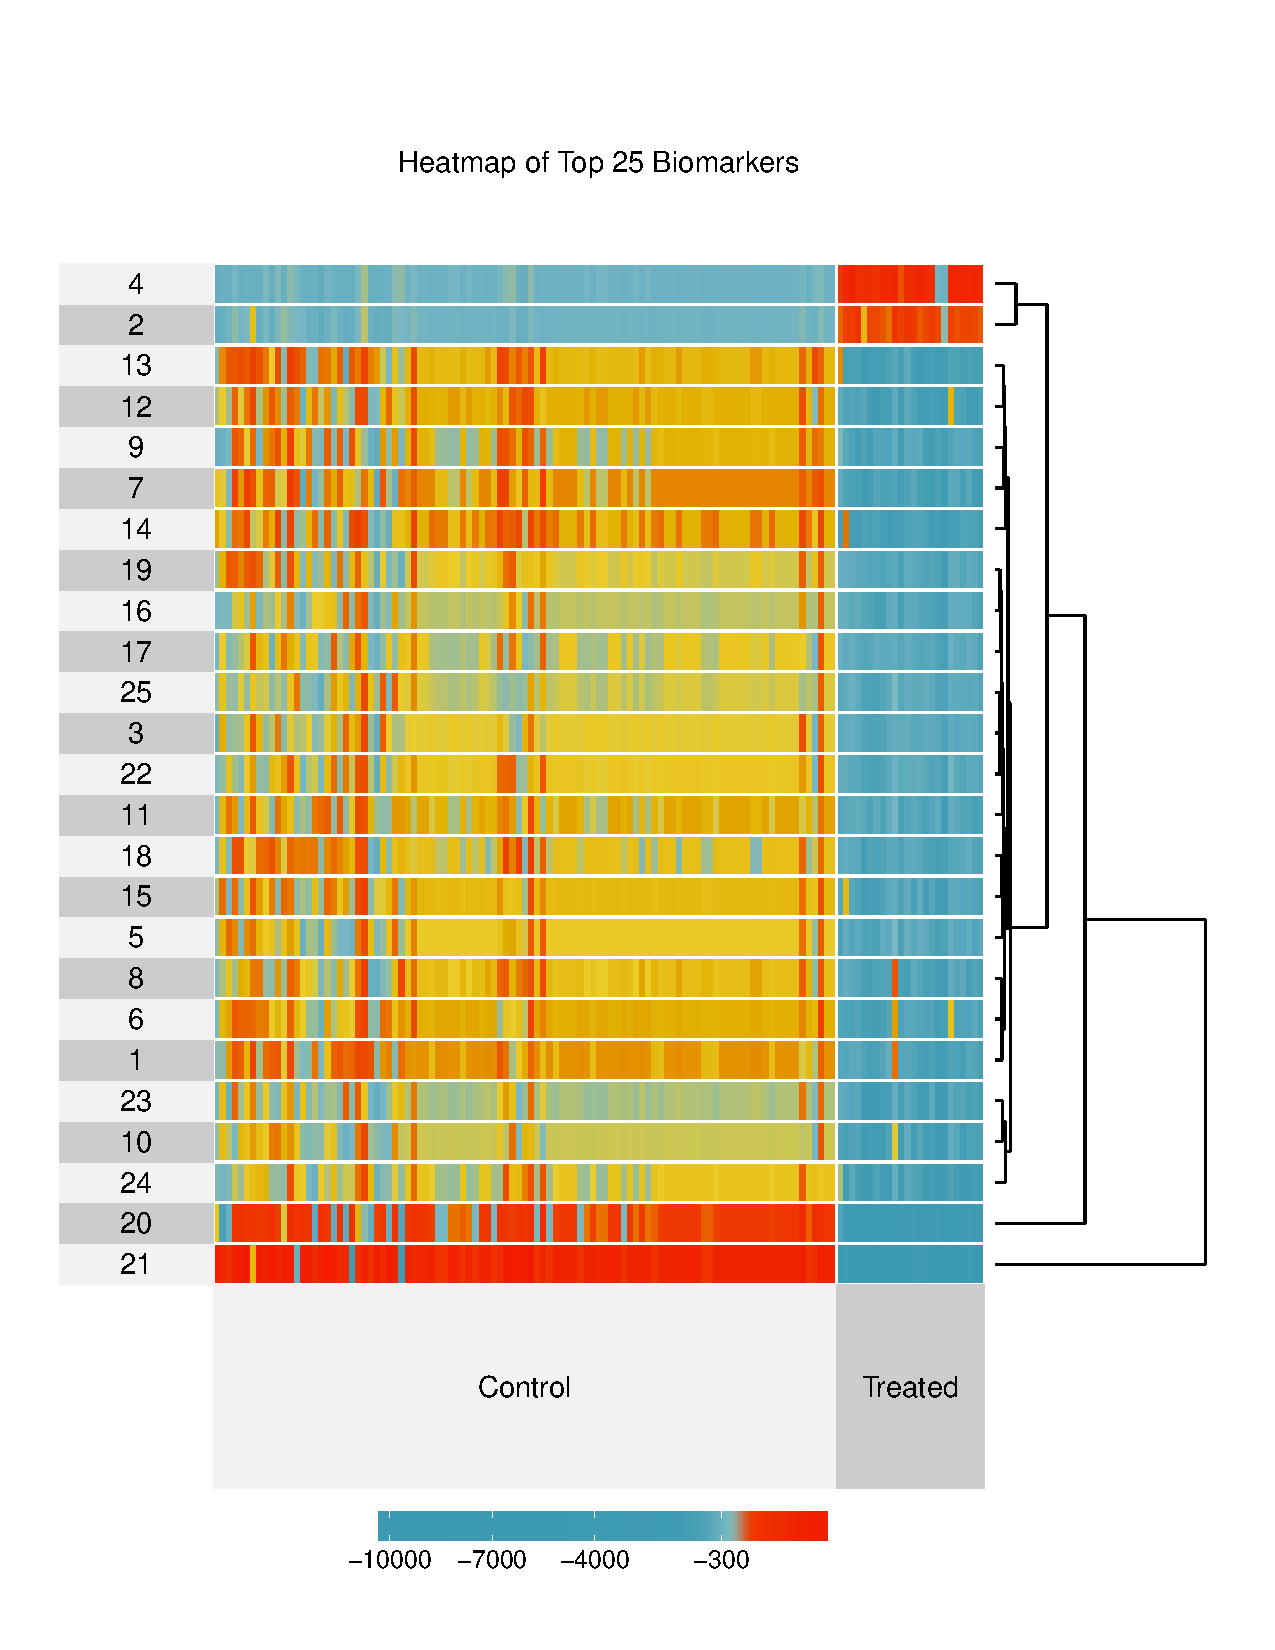
\includegraphics[scale=0.75]{superheatmap.pdf}
  \caption{Heatmap of the ATE estimates. Blue indicates a depression in the
    ATE, while red indicates an increase in the ATE, based on exposure to the
    maximal level of benzene as opposed to the minimal level.}
\end{figure}

As expected, Limma reduced the spread of the standard deviation estimates of
the the influence curve by probe ($\widetilde{\sigma}^b_n$) across the
$\sim 20,000$ probes, and the corresponding Wald statistics for testing the
target parameter, in comparison of using the original standard error,
$\sigma^b_n$. The results of our analysis indicate that the moderated
t-statistic applied to the ATE constitutes a powerful approach for assessing
variable importance, based on exposure, in the context of high-dimensional
investigations of biomarkers. We conclude that using this adaptation of TMLE,
complimented by the moderated t-statistic of the R package LIMMA, reduces the
variability of standard errors and reduces the number of significant probes,
leading to more stable and robust inference, while providing the opportunity to
evaluate biomarkers in the context of statistical parameters of scientific
relevance, such as the average treatment effect focused on in the above example.
